\section*{Problema 19 del Capítulo 4}

\textbf{Enunciado:}
Describir lo mejor que se pueda las gráficas de las siguientes funciones (una descripción completa es, por lo general, imposible):

\begin{enumerate}
    \item $f(x) =$ el primer número del desarrollo decimal de $x$.
    \item $f(x) =$ el segundo número del desarrollo decimal de $x$.
    \item $f(x) =$ el número de sietes del desarrollo decimal de $x$ si este número es finito, y $0$ en el caso contrario.
    \item $f(x) = 0$ si el número de sietes en el desarrollo decimal de $x$ es finito y $1$ en el caso contrario.
    \item $f(x) =$ el número obtenido sustituyendo todas las cifras del desarrollo decimal de $x$ que vienen después del primer $7$ (si las hay) por $0$.
\end{enumerate}

\textbf{Demostración:}

\begin{enumerate}
    \item \textbf{Primera función:} $f(x) =$ el primer número del desarrollo decimal de $x$.
    
    La gráfica de esta función consiste en una serie de segmentos horizontales. Cada segmento corresponde a un intervalo de números reales que comparten el mismo primer dígito en su desarrollo decimal. Por ejemplo, para $f(x) = 1$, el intervalo es $[1, 2)$, para $f(x) = 2$, el intervalo es $[2, 3)$, y así sucesivamente hasta $f(x) = 9$ con el intervalo $[9, 10)$.

    \begin{figure}[h!]
    \centering
    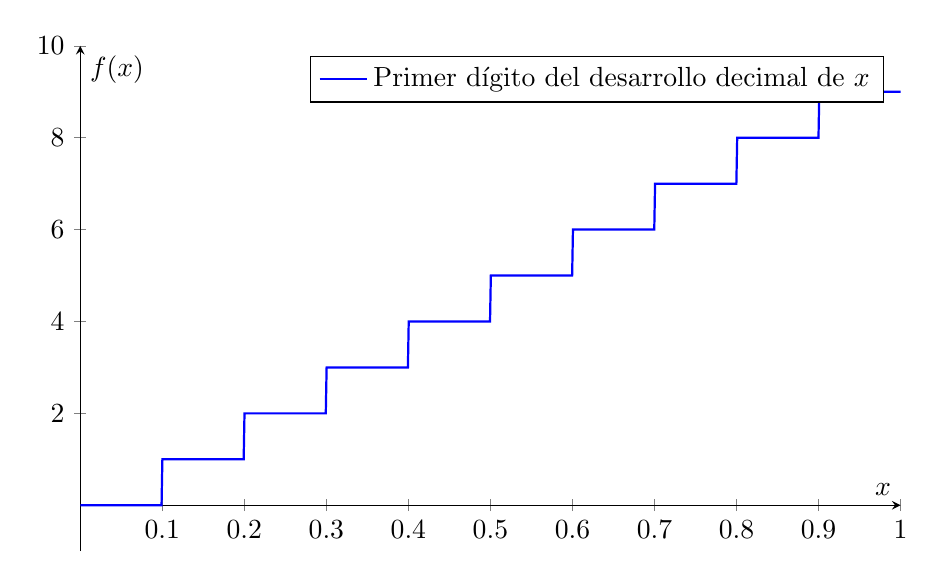
\begin{tikzpicture}
        \begin{axis}[
            axis lines = middle,
            xlabel = $x$,
            ylabel = {$f(x)$},
            ymin = -1, ymax = 10,
            xmin = 0, xmax = 1,
            samples = 1000,
            domain = 0:1,
            width=12cm,
            height=8cm
        ]
        \addplot[blue, thick] {floor(x*10)};
        \addlegendentry{Primer dígito del desarrollo decimal de $x$}
        \end{axis}
    \end{tikzpicture}
    \caption{Gráfica de $f(x)$ para el primer dígito del desarrollo decimal de $x$.}
    \label{fig:primer_digito}
    \end{figure}

    \item \textbf{Segunda función:} $f(x) =$ el segundo número del desarrollo decimal de $x$.
    
    Similar a la primera función, la gráfica de esta función también consiste en segmentos horizontales. Sin embargo, estos segmentos son más pequeños, ya que dependen del segundo dígito del desarrollo decimal. Por ejemplo, para $f(x) = 1$, los intervalos son $[0.1, 0.2)$, $[1.1, 1.2)$, $[2.1, 2.2)$, etc.

    \item \textbf{Tercera función:} $f(x) =$ el número de sietes del desarrollo decimal de $x$ si este número es finito, y $0$ en el caso contrario.
    
    La gráfica de esta función es más compleja. Para los números racionales, el desarrollo decimal es finito o periódico, por lo que $f(x)$ será un número finito. Para los números irracionales, el desarrollo decimal no es periódico, y $f(x) = 0$.

    \item \textbf{Cuarta función:} $f(x) = 0$ si el número de sietes en el desarrollo decimal de $x$ es finito y $1$ en el caso contrario.
    
    Esta función es una función indicadora que toma el valor $0$ para los números racionales (donde el número de sietes es finito) y $1$ para los números irracionales (donde el número de sietes es infinito).

    \item \textbf{Quinta función:} $f(x) =$ el número obtenido sustituyendo todas las cifras del desarrollo decimal de $x$ que vienen después del primer $7$ (si las hay) por $0$.
    
    La gráfica de esta función es discontinua en los puntos donde aparece el primer $7$ en el desarrollo decimal de $x$. En estos puntos, la función cambia abruptamente, ya que todas las cifras después del primer $7$ se convierten en $0$.

    \item \textbf{Sexta función:} $f(x) = 0$ si $1$ no aparece en el desarrollo decimal de $x$, y $n$ si $1$ aparece por primera vez en el $n$-ésimo lugar.
    
    La gráfica de esta función es discontinua y depende de la posición del primer $1$ en el desarrollo decimal de $x$. Para los números racionales que no contienen el dígito $1$, $f(x) = 0$. Para los números que contienen el dígito $1$, la función toma valores enteros positivos dependiendo de la posición del primer $1$.
\end{enumerate}

\end{document}